\begin{frame}
	\frametitle{Motivation}
	\begin{itemize}
		\item Chicago alderman have substantial power to shape local land use and development decisions
		\item It has received increased scrutiny in recent years, from both local politicians and the federal government \\ 
		{\scriptsize \cite{chase_chicago_2023,freemark_zoning_2024}}
		\item Very little existing work on the effects of this unique power on development outcomes \\
		{\scriptsize \cite{khan_decentralized_2021}}
	\end{itemize}
\end{frame}


\begin{frame}
	\frametitle{Aldermanic Privilege is a Hotly Contested Issue in Chicago} 
    \begin{minipage}{0.5\textwidth}
        \begin{figure}
            \centering
            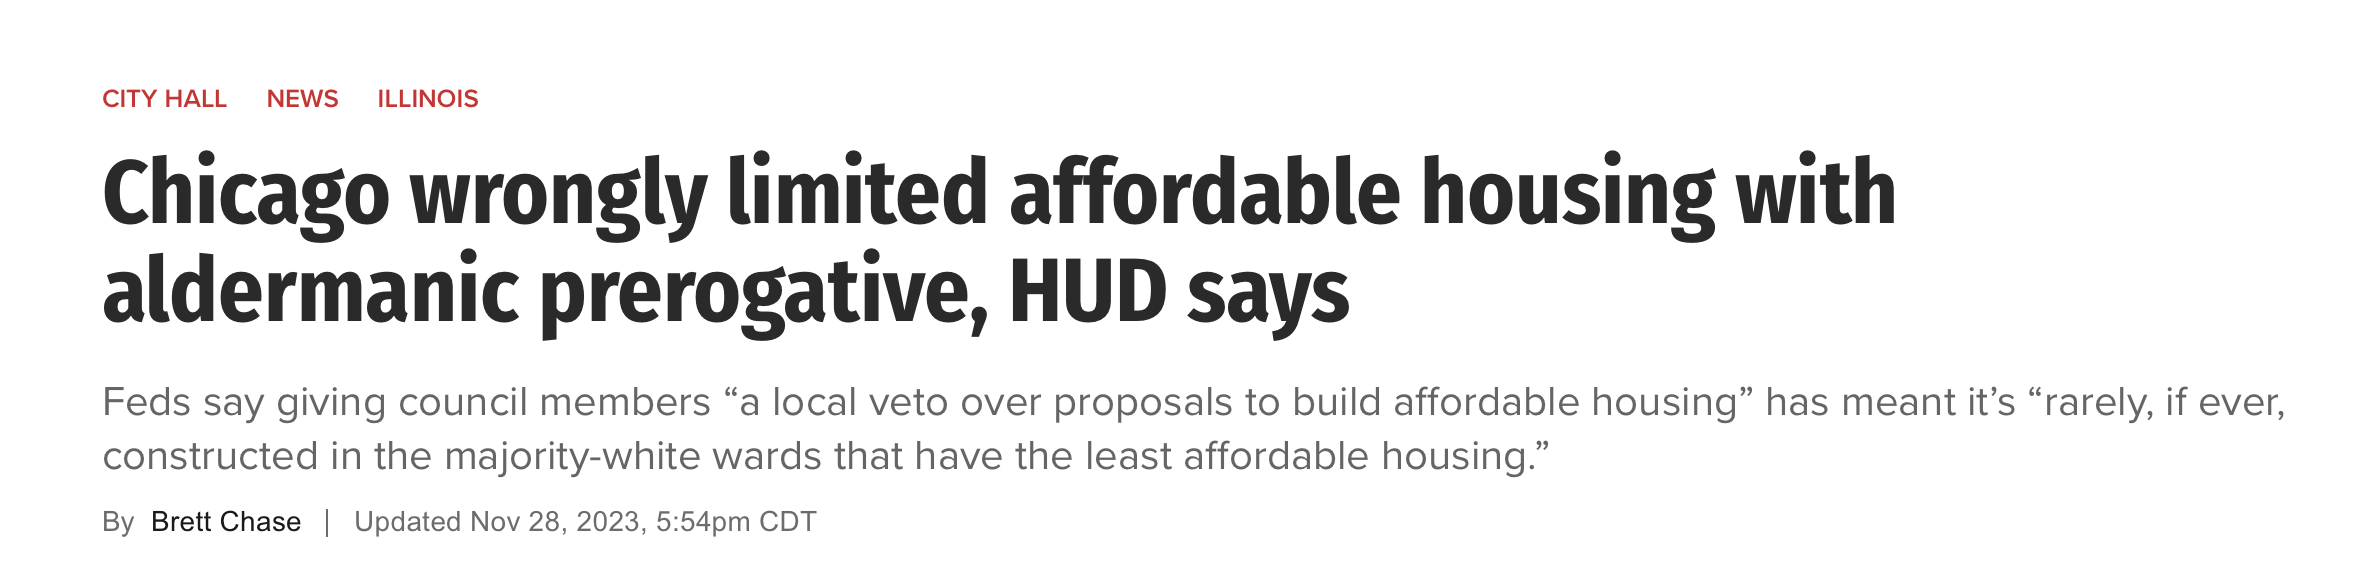
\includegraphics[width=\textwidth]{images/hud_report_headline.png}
		\end{figure}
		\begin{figure}
			\centering
			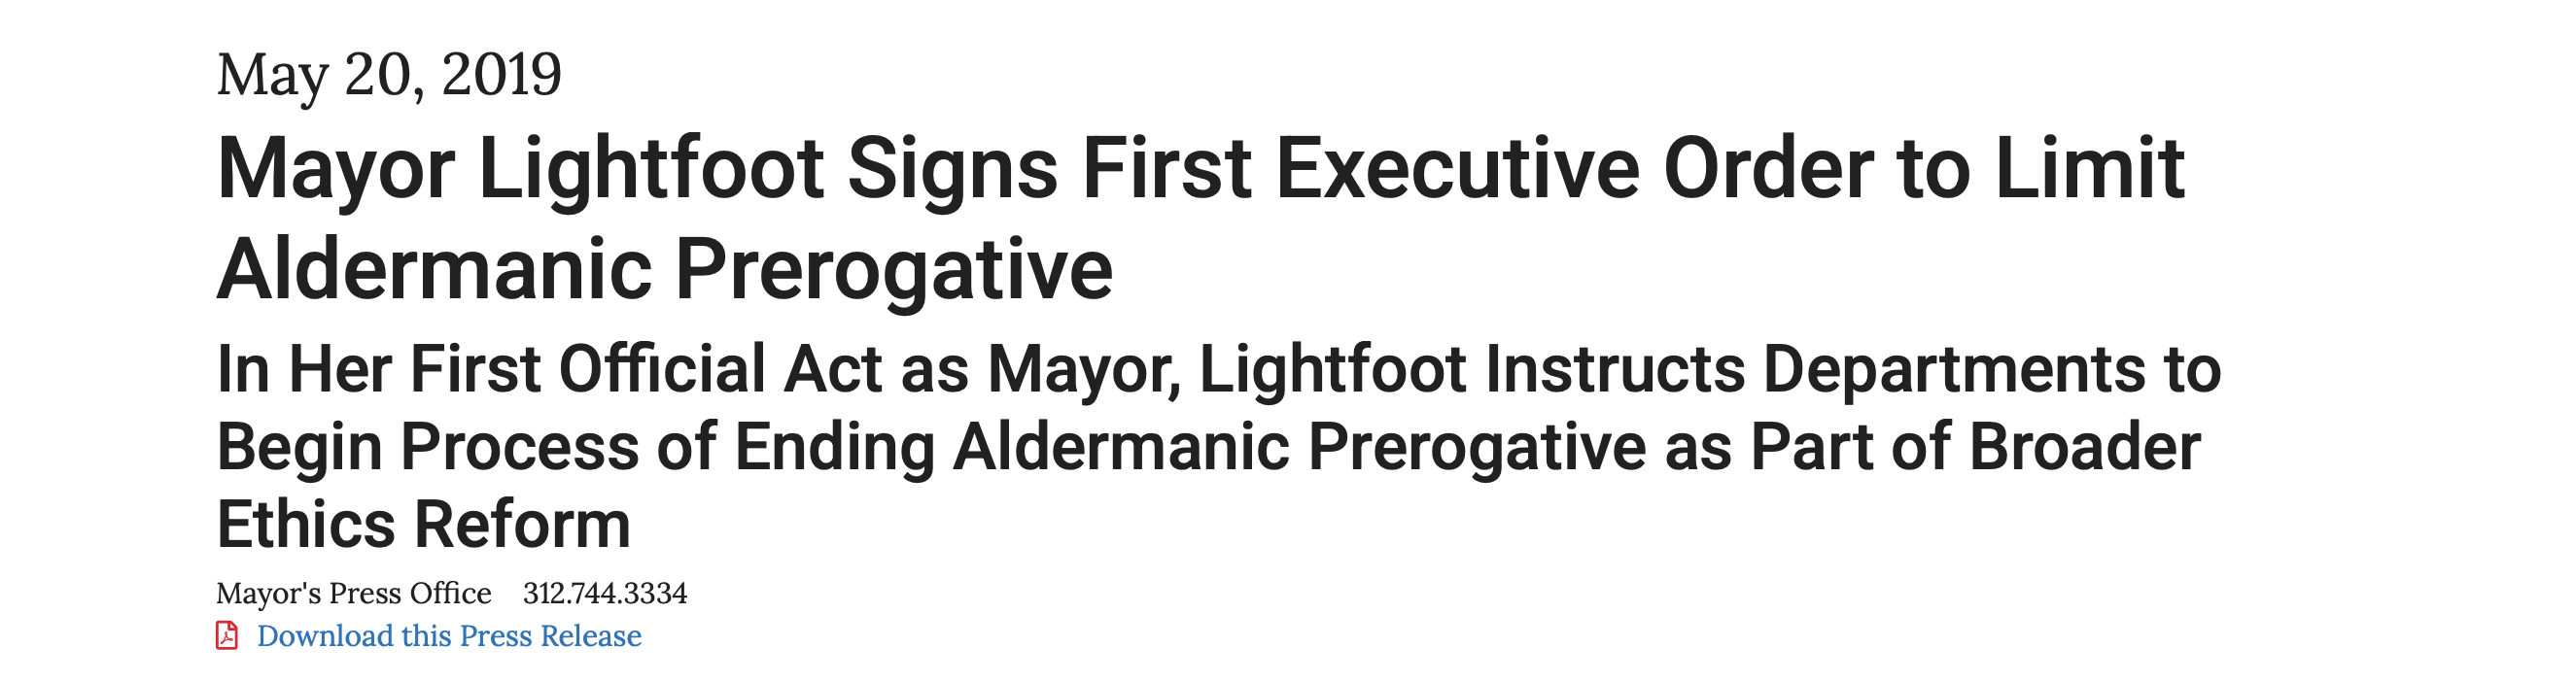
\includegraphics[width=\textwidth]{images/lightfoot_order.png}
		\end{figure}
		\begin{figure}
			\centering
			
\includegraphics[width=\textwidth]{images/alderman_fight.png}
		\end{figure}
        \end{minipage}
        \hfill
        \begin{minipage}{0.48\textwidth}
        \begin{figure}
            \centering
            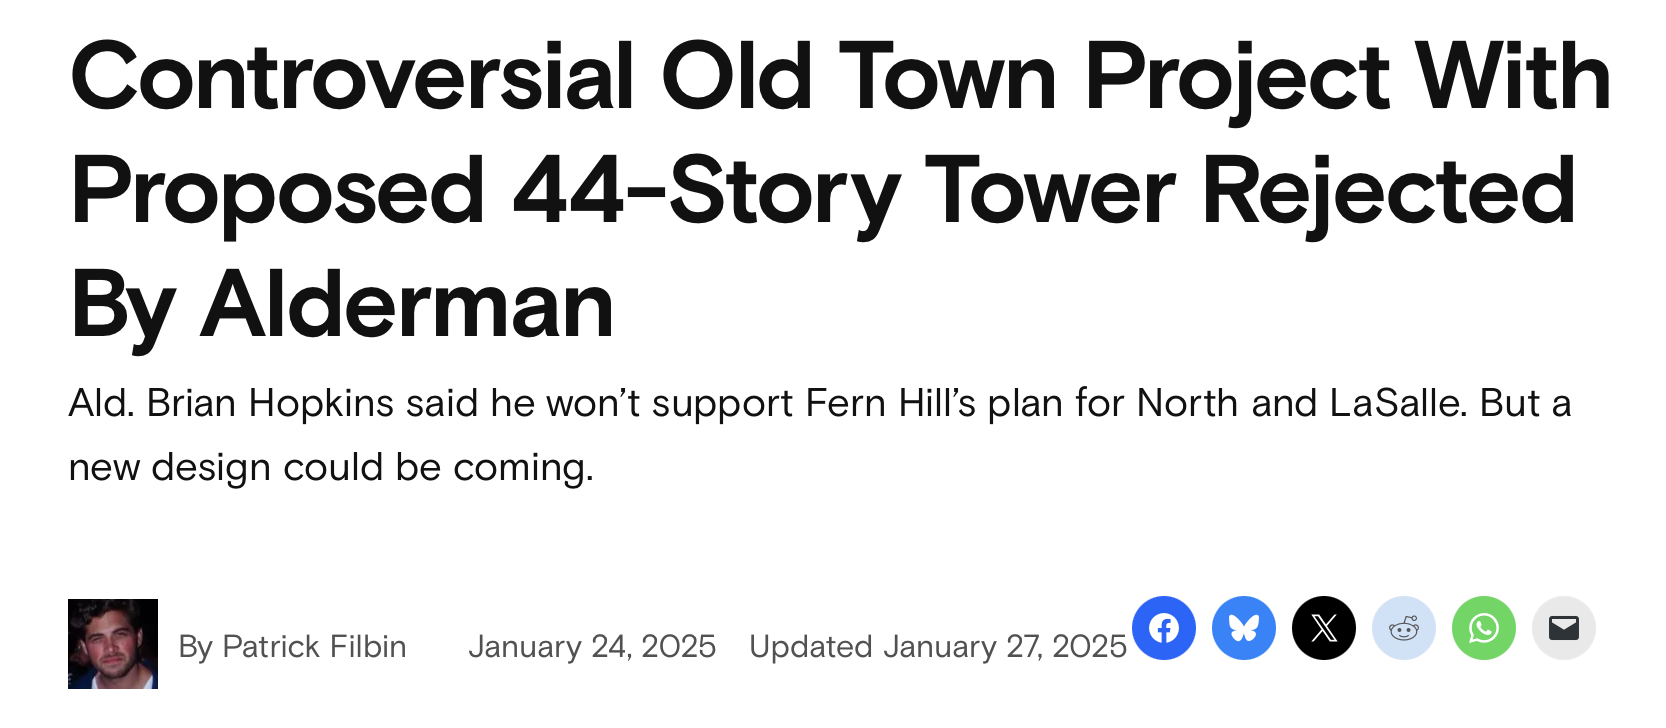
\includegraphics[width=\textwidth]{images/old_town_towers.png}
		\end{figure}
		\begin{figure}
			\centering
			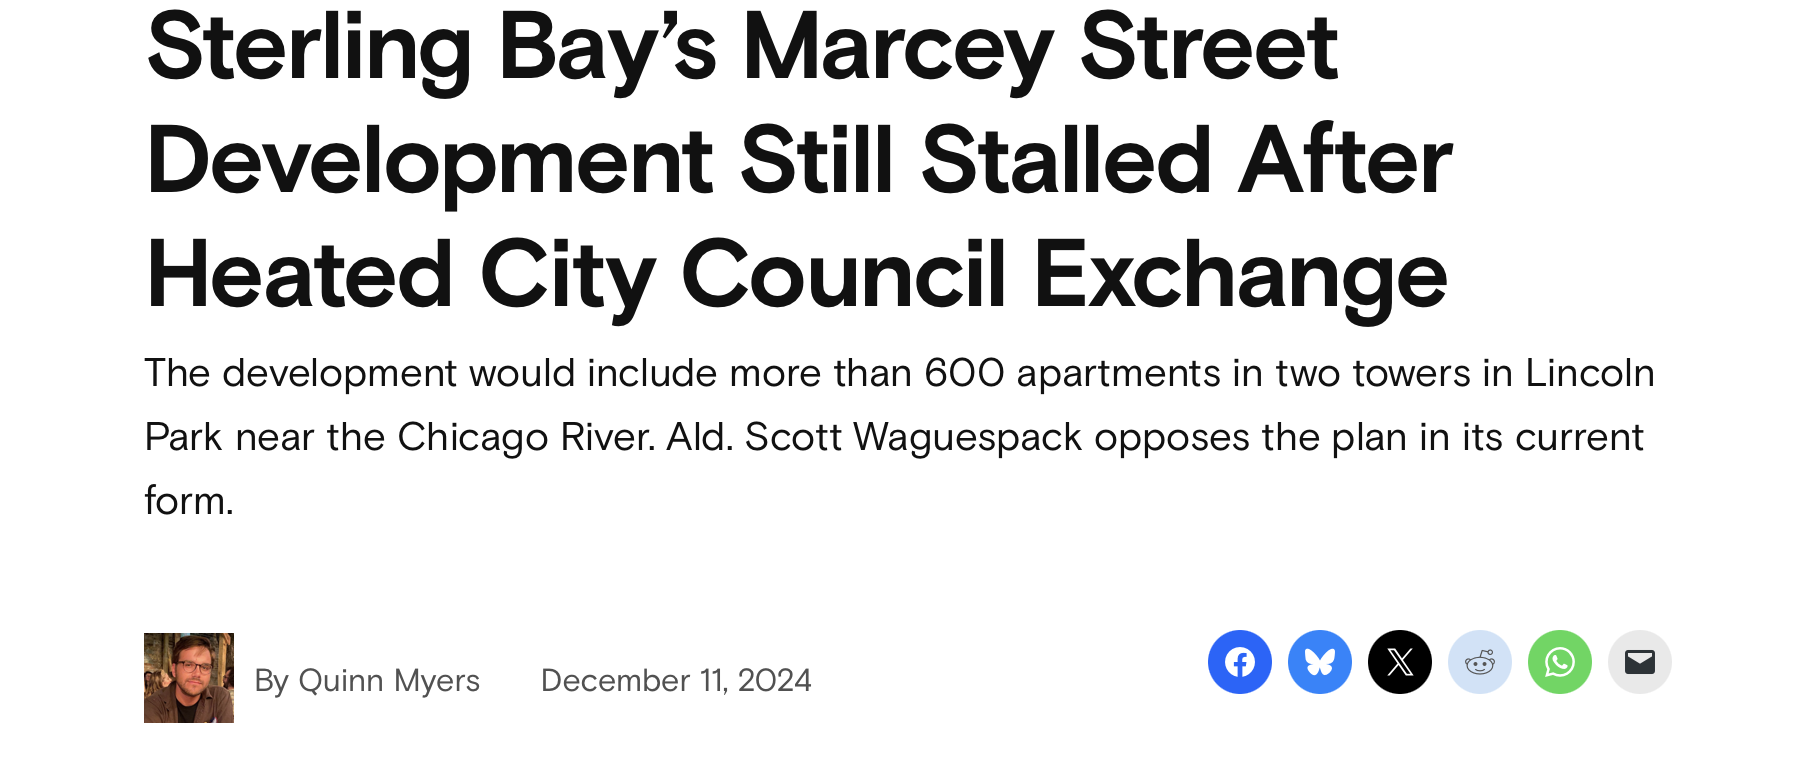
\includegraphics[width=\textwidth]{images/sterling_bay_fight.png}
        \end{figure}
        \end{minipage}
\end{frame}

\begin{frame}
	\frametitle{Preview of Results}
	\begin{itemize}
		\item I find that aldermanic privilege reduces the Floor Area Ratio (FAR) of new developments by $40\%$ within $.1$ miles of the ward boundary, with the effect diminishing with distance from the ward border
		\begin{itemize}
			\item This result is robust to using alternative density measures such as Lot Area Per Unit (LAPU), Bulding Coverage Ratio (BCR), and Lot Size Per Story (LPS)
			\item It is also robust to many bandwidth choices, kernels, and functional forms of the RD
		\end{itemize}
		\item I find similar results using a ward-border-pair fixed effects approach 
	\end{itemize}
\end{frame}

\begin{frame}
	\frametitle{Roadmap}
	\begin{itemize}
		\item Literature Review
		\item Data 
		\item Alderman Fixed Effects
		\item Descriptive Bunching Analysis
		\item Spatial RD Results
		\item Border-Pair Fixed Effects Results
	\end{itemize}
\end{frame}